\section{Test Results: PWM \& Buck Converter}
%Include test results (e.g. oscilloscope traces) which show that the converter operates correctly and satisfies the specifications. The results from the tests should be compared to the simulation results. Note the earlier simulations results may have to be changed to match the actual test conditions.

\begin{figure}
	\centering
	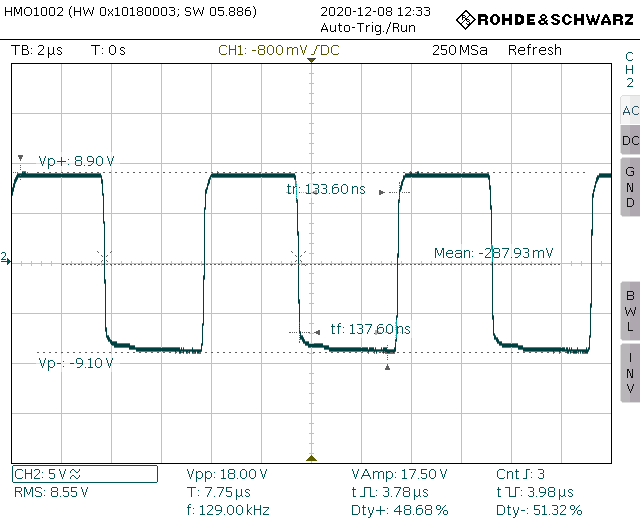
\includegraphics[width=\linewidth]{CARRYB05.PNG}
	\caption{Output voltage of PWM circuit when disconnected from converter.}
	\label{fig:test vg}
\end{figure}

\begin{figure}
	\centering
	\includegraphics[width=\linewidth]{"img/test VoVg"}
	\caption{Converter output voltage (top) and PWM output voltage (bottom) for RL = $\SI{4.7}{\ohm}$.}
	\label{fig:test-vovg}
\end{figure}


\begin{figure}
	\centering
	\includegraphics[width=\linewidth]{"img/test Vo Vg max"}
	\caption{Maximum duty cycle}
	\label{fig:test-vo-vg-max}
\end{figure}

\begin{figure}
	\centering
	\includegraphics[width=\linewidth]{"img/test Vo Vg min"}
	\caption{Minimum duty cycle}
	\label{fig:test-vo-vg-min}
\end{figure}

\Cref{fig:test-vovg} gives the converter and PWM output voltages or $R_L = \SI{4.7}{\ohm}$.

\Cref{fig:test vg} gives the PWM output voltage before connecting the two circuits. Note the lack of distortion.

%In addition to presenting the test results include an answer to the following questions:

\subsection{Do the test results and the simulation results agree?}
% Comment on the results and especially any disagreement and the possible reasons for the disagreement.
The switching frequency varied from \SI{125}{\kilo\hertz} to \SI{135}{\kilo\hertz}. It seemed to increase the longer we had the circuit on, possibly indicating some temperature dependency; this could also be due to one of us moving components on the breadboard and causing changes in capacitance.
The initially high value for the switching frequency could be due to the choice of RC product initially. The simulation switching frequency was quite different, at \SI{90}{\kilo\hertz}, indicating that the fault might be elsewhere.

The output voltage was \SI{4}{\volt}, four fifths of the specification. The simulated output voltage of 4.7 V is much closer to desired.

The large amount of distortion present in the converter output voltage could be caused by some feedback created when the two circuits were connected (\cref{fig:test vg} shows the gate voltage before connection). This would have affected the reference input also, reducing the range of duty cycles available to the controller.
\subsection{Provide a plot of converter output voltage vs. PWM reference voltage. Is this relationship as expected?}
% Comment and explain.
\Cref{fig:test-vo-vg-max,fig:test-vo-vg-min} give the PWM and converter output voltages for the maximum and minimum duty cycles we achieved. There is not a great range of duty cycles due to distortion of the reference voltage. The duty cycle was adjusted by varying the reference voltage. This relationship is not what we had expected, we had expected a relatively linear relationship that would allow for a much wider range of duty cycles.
\subsection{How does the measured efficiency compare with the simulated efficiency and calculated efficiency?}
% Comment and explain any differences.
The efficiency of the circuit was calculated by measuring the current and voltage provided by the various supplies ($\SI{0.05}{\ampere}\cdot\SI{10}{\volt}+\SI{0.05}{\ampere}\cdot\SI{10}{\volt}+\SI{0.4}{\ampere}\cdot\SI{10}{\volt}=\SI{5}{\watt}$) and dividing the dissipated load power by it ($\frac{4^2}{4.7}=\SI{3.4}{\watt}$) giving an efficiency of 68\%. This is somewhat less than the simulated value of 86\%, but rather close to the calculated efficiency of 65\%. Differences could be due to, among other factors, larger losses in the inductor due to the distortion.
